\documentclass[10pt,letterpaper,twoside]{article}
\usepackage{code/manuscript_assets/researchpreprint}
\usepackage{amsmath,amssymb,amsthm,mathtools,bm,booktabs,graphicx,xcolor,placeins,xurl}
\newcommand{\ResultRows}{%
Si2 & 769 & 6 & 24 & 1.40e-04 & 6.87e-16 & 144 & 1.36 \\
SiH4 & 5,041 & 5 & 24 & 2.09e-04 & 3.23e-15 & 120 & 1.65 \\
benzene & 8,219 & 6 & 24 & 1.39e-04 & 1.74e-15 & 144 & 2.04 \\
Si5H12 & 19,896 & 6 & 24 & 1.47e-04 & 1.24e-15 & 144 & 0.99 \\}
\newcommand{\DataRows}{%
Si2 & 769 & 17,801 & development & 0.979996 \\
SiH4 & 5,041 & 171,903 & confirmation & 0.980000 \\
benzene & 8,219 & 242,669 & confirmation & 0.980000 \\
Si5H12 & 19,896 & 738,598 & confirmation & 0.980000 \\}
\newcommand{\AblationRows}{%
Si2 & 1.36 & 3.12 & 3.88 \\
SiH4 & 1.65 & 1.97 & 7.59 \\
benzene & 2.04 & 1.89 & 10.67 \\
Si5H12 & 0.99 & 1.33 & 5.28 \\}
\newcommand{\SemanticDigest}{eae62cf6af1c}

\newcommand{\RR}{\mathbb{R}}
\newcommand{\norm}[1]{\left\lVert #1\right\rVert}
\newcommand{\ip}[2]{\left\langle #1,#2\right\rangle_F}
\newcommand{\Lfrechet}{\mathcal{L}}
\newcommand{\Krylov}{\mathcal{K}}
\newcommand{\Br}{B_r}
\newcommand{\Fhat}{\widehat F}
\newcommand{\ghat}{\widehat g}
\newtheorem{theorem}{Theorem}
\newtheorem{lemma}{Lemma}
\newtheorem{corollary}{Corollary}
\begin{document}
\title{Certified Rank--Depth Selection for Block Matrix-Function Gradients}
\author{Molena Huynh}
\email{molena.huynh@jmp.com}
\affiliation{North Carolina State University}
\date{September 15, 2026}
\maketitle
\begin{abstract}
Inverse problems with correlated preparations require block matrix-function
responses and parameter derivatives. For cosine responses of symmetric affine
operators, we derive a loss-aware compression bound whose retained-block
contribution cancels, giving quadratic dependence on the discarded probe norm
for consistent targets. Separate response and operator-derivative Chebyshev
remainders bound the inexact loss gradient before operator applications. A
finite search minimizes nominal Hamiltonian-vector work $mr$ over certified
rank--depth pairs. On four authenticated electronic-structure Hamiltonians of
orders 769--19,896, the refinements reduce joint certified work from 120 to 48
vector applications, a 60 percent saving; independent gradient discrepancies
are below $9\times10^{-9}$ at tolerance $10^{-3}$. Certification nevertheless
costs more than an incremental full-block stopping heuristic at that tolerance.
A larger simulated inverse study crosses two chain sizes, three truths, two
starts, two noisy realizations plus clean data, two stationarity targets, and
four methods. All 288 runs recover parameters within $10^{-3}$, with active
compression during certified feasible-descent iterations. Strict final
stationarity can require full probe rank and remove the work benefit. The
original 96-site recovery failures are retained and diagnosed independently.
The results establish a sharper exact-arithmetic resource guarantee and
reduced learning computations, while separating these benefits from runtime,
finite-precision certification, and global identifiability.
\end{abstract}

\section{Introduction}
Matrix-function inverse problems arise in quantum dynamics, response calculations,
and scientific computing \cite{higham2008,saad1992,hochbruck1997}. For a large
symmetric operator $A(\theta)$ and a thin preparation block $B$, the observations
may involve every entry of $B^{\mathsf T}f(A(\theta))B$. Correlated columns create
an opportunity to reduce the width of each operator application. The difficulty
is to account for the resulting perturbation of the loss gradient while also
choosing a sufficient Krylov depth.

Block Krylov projection and its matrix-function error analysis are established
\cite{gutknecht2007,xu2022,chen2022}. Fr\'echet derivatives admit augmented,
low-rank, and bivariate Krylov formulations
\cite{kandolf2017,kandolf2021,kressner2019}. Singh, Barros, and Li
\cite{singh2026} develop a forward-only gradient approximation for Hermitian
bilinear forms, including learning examples. Scalar bilinear responses can
also be reconstructed by polarization, so block output alone does not define
the novelty of the present method.

Our contribution is a resource-selection guarantee for cosine block gradients
that combines a loss-aware compression bound with separate response and
operator-derivative Chebyshev tails. The supporting norm inequalities are
elementary; their integration permits a finite search
over rank and depth without extending the large Krylov space. We distinguish
response exactness through degree $2m-1$ from derivative exactness through
$m$, and minimize $mr$ over feasible pairs. This is a grid optimum for the
specified work model, not a minimum-runtime theorem.

The experiments answer three separate questions: whether compression reduces
work at the same depth; whether it reduces work at the same certified tolerance;
and whether certification is competitive with methods that achieve the same
observed accuracy. A simulated lattice inverse problem then tests whether the
inexact gradients support parameter recovery. Authentic Hamiltonian inputs,
constructed numerical probes, and simulated physical observations are explicitly
distinguished. No quantum computational advantage is claimed.

\section{Objective and access model}
Let $A(\theta)=H_0+\sum_{j=1}^p\theta_jD_j$ be real symmetric, with
$|\theta_j|\le a_j$, and let $B\in\RR^{n\times b}$. Define
\begin{equation}
 F_\ell(\theta)=B^{\mathsf T}\cos(t_\ell A(\theta))B,\qquad
 \Phi(\theta)=\frac1{2s}\sum_{\ell=1}^s\norm{F_\ell-Y_\ell}_F^2.
 \label{eq:objective}
\end{equation}
The exact gradient is
\begin{equation}
 g_j=\frac1s\sum_\ell\ip{F_\ell-Y_\ell}
 {B^{\mathsf T}\Lfrechet_{f_\ell}(A,D_j)B},\quad f_\ell(x)=\cos(t_\ell x).
 \label{eq:gradient}
\end{equation}
Here $\Lfrechet_f$ is the Fr\'echet derivative \cite{higham2008,al-mohy2009}.
The implementation needs block actions of $A$ and of each $D_j$. Diagonal
fields and symmetric sparse off-diagonal directions are supported.

\begin{lemma}[Uniform enclosure]
If $\norm{H_0}_\infty+\sum_j a_j\norm{D_j}_2\le\rho$, then
$\norm{A(\theta)}_2\le\rho$ on the entire parameter box.
\end{lemma}
\begin{proof}
Symmetry implies $\norm{H_0}_2\le\norm{H_0}_\infty$. Apply the triangle
inequality and $|\theta_j|\le a_j$. A diagonal direction has spectral norm
$\max_i|(D_j)_{ii}|$; the maximum absolute row sum bounds a symmetric sparse
direction's spectral norm.
\end{proof}
No eigenvalue iteration is required. This is an exact-arithmetic statement;
floating-point row sums are not interval enclosures. The cosine analysis does
not require $\rho<1$: the approximation difficulty depends on $|t|\rho$.
Rescaling a physical Hamiltonian by $c$ must be accompanied by rescaling time
by $1/c$ to preserve the evolution. The PARSEC times below are dimensionless
benchmark inputs, not experimental times.

\section{Compression, projection, and certification}
\subsection{Probe compression}
Write the thin SVD as $B=U\Sigma W^{\mathsf T}$ and its rank-$r$ truncation
as $B_r=U_r\Sigma_rW_r^{\mathsf T}=C_rW_r^{\mathsf T}$. Let
$\delta_r=\norm{B-B_r}_F$ and $\alpha_r=2\norm B_2\delta_r$.
\begin{theorem}[Compression perturbation]
For real symmetric $A,D$,
\begin{align}
 \norm{B^{\mathsf T}\cos(tA)B-B_r^{\mathsf T}\cos(tA)B_r}_F&\le\alpha_r,\\
 \norm{B^{\mathsf T}\Lfrechet_{f_t}(A,D)B-B_r^{\mathsf T}\Lfrechet_{f_t}(A,D)B_r}_F
 &\le |t|\norm D_2\alpha_r.
\end{align}
\end{theorem}
\begin{proof}
Put $E=B-B_r$. For any $M$,
$B^{\mathsf T}MB-B_r^{\mathsf T}MB_r=E^{\mathsf T}MB+B_r^{\mathsf T}ME$.
Frobenius--spectral product inequalities bound its norm by
$(\norm B_2+\norm{B_r}_2)\norm M_2\delta_r=\alpha_r\norm M_2$.
For $M=\cos(tA)$ the norm is at most one. Differentiating $e^{it(A+sD)}$
by the Duhamel formula and using unitary invariance gives
$\norm{\Lfrechet_{e^{it(\cdot)}}(A,D)}_2\le|t|\norm D_2$.
Averaging the two exponential derivatives proves the cosine bound.
\end{proof}
Set $c_B=\norm B_2\norm B_F$ and $c_r=\norm{B_r}_2\norm{B_r}_F$.
The exact and compressed exact gradients differ componentwise by at most
\begin{equation}
 \chi_{j,r}=\frac{\alpha_r\norm{D_j}_2}{s}
 \sum_\ell |t_\ell|(c_B+c_r+\norm{Y_\ell}_F).
 \label{eq:chi}
\end{equation}
This follows by adding and subtracting the compressed response times the full
derivative in Eq.~\eqref{eq:gradient}, then applying the preceding theorem.

The loss permits a sharper estimate because its retained--retained gradient
contribution cancels exactly. Complete $W_r$ to an orthogonal matrix
$[W_r\ W_d]$, put $C_d=BW_d$, and define
$u_r=\norm{C_r}_2\norm{C_d}_F$ and
$v_r=\norm{C_d}_2\norm{C_d}_F$. Zero singular components may be included in
$C_d$ when $b>n$. Assume the targets are symmetric, as are the observations.
For nonsymmetric targets, their symmetric parts give the same gradient.
\begin{theorem}[Loss-aware compression]
Writing $Y_{\ell,rd}=W_r^{\mathsf T}Y_\ell W_d$ and
$Y_{\ell,dd}=W_d^{\mathsf T}Y_\ell W_d$, one has
\begin{equation}
 |g_j-g_j^{(r)}|\le \widetilde\chi_{j,r}:=
 \frac{\norm{D_j}_2}{s}\sum_\ell |t_\ell|
 \left[2u_r(u_r+\norm{Y_{\ell,rd}}_F)
 +v_r(v_r+\norm{Y_{\ell,dd}}_F)\right].
 \label{eq:loss-aware}
\end{equation}
For consistent noiseless targets $Y_\ell=B^{\mathsf T}\cos(t_\ell A_\star)B$,
the bracket is at most $4u_r^2+2v_r^2$.
\end{theorem}
\begin{proof}
Transform both factors of the Frobenius inner product in
Eq.~\eqref{eq:gradient} by $[W_r\ W_d]$. The retained--retained terms are
identical for $B$ and $B_r$; the difference consists of twice the
retained--discarded term and the discarded--discarded term. Their response
norms are at most $u_r,v_r$, and their derivative norms at most
$|t_\ell|\norm{D_j}_2u_r,|t_\ell|\norm{D_j}_2v_r$. Cauchy--Schwarz gives
Eq.~\eqref{eq:loss-aware}. Consistent target blocks obey the same response
bounds. Thus the consistent-target bound is quadratic in the discarded
probe norm; arbitrary noise is handled by the actual target blocks.
\end{proof}
The default compression bound is
$\bar\chi_{j,r}=\min\{\chi_{j,r},\widetilde\chi_{j,r}\}$ componentwise.
The linear bound is retained as an
ablation. Target block norms are evaluated with
$P_d=I-W_rW_r^{\mathsf T}$, avoiding an additional orthogonal completion.

\subsection{Distinct response and derivative exactness}
Let $m\ge2$ and define $\Krylov_m(A,C_r)=\operatorname{span}\{C_r,AC_r,\ldots,A^{m-1}C_r\}$.
Let $V$ be an orthonormal basis of this space, and
write $T=V^{\mathsf T}AV$, $C=V^{\mathsf T}C_r$, and $Q=CW_r^{\mathsf T}$.
The lifted approximations are
\begin{equation}
 \Fhat_\ell=Q^{\mathsf T}\cos(t_\ell T)Q,\quad
 \widehat J_{\ell j}=Q^{\mathsf T}\Lfrechet_{f_\ell}
 (T,V^{\mathsf T}D_jV)Q,\quad
 \ghat_j=\frac1s\sum_\ell\ip{\Fhat_\ell-Y_\ell}{\widehat J_{\ell j}}.
 \label{eq:estimator}
\end{equation}
We call $\ghat$ an \emph{inexact gradient of the original loss}. It generally
is not the derivative of the computed projected loss when rebuilding $V$ as
$\theta$ changes; that derivative also contains basis-variation terms.

\begin{theorem}[Polynomial exactness]
The identity $C_r^{\mathsf T}q(A)C_r=C^{\mathsf T}q(T)C$ holds for every
polynomial of degree at most $2m-1$. The identity
$C_r^{\mathsf T}\Lfrechet_q(A,D)C_r
=C^{\mathsf T}\Lfrechet_q(T,V^{\mathsf T}DV)C$ holds for degree at most $m$.
\end{theorem}
\begin{proof}
For $0\le k\le m-1$, $A^kC_r=VT^kC$. For a response monomial of degree
at most $2m-2$, split the degree into two powers at most $m-1$ and use symmetry.
For degree $2m-1$, use
$(A^{m-1}C_r)^{\mathsf T}A(A^{m-1}C_r)=C^{\mathsf T}T^{2m-1}C$.
For a derivative monomial of degree $k\le m$,
$\Lfrechet_{x^k}(A,D)=\sum_{u=0}^{k-1}A^uDA^{k-1-u}$; both powers are at
most $m-1$, so substitution proves the identity term by term. Linearity
completes the proof. The derivative assertion does not in general extend to
$2m-1$.
\end{proof}

\begin{corollary}[Invariant-space termination]
If $AV=VT$ and $C_r$ lies in the range of $V$, both compressed responses and
sandwiched derivatives are exact for cosine. In particular this holds when
$V$ is square and orthogonal.
\end{corollary}
\begin{proof}
Invariance gives $A^kC_r=VT^kC$ for every $k$. Apply the monomial derivative
identity termwise to the absolutely convergent cosine series.
\end{proof}
This statement concerns exact invariance. A small numerical factorization
residual is not by itself a proof of zero error; the implementation removes
the projection tail only for a square computed basis, under its stated
exact-arithmetic interpretation.

\subsection{Gradient certificate}
For $\rho>0$, define the positive Taylor tails
\begin{equation}
 R_d^{(0)}(t,\rho)=\sum_{\substack{\nu>d\\\nu\ \mathrm{even}}}\frac{|t|^\nu\rho^\nu}{\nu!},\qquad
 R_d^{(1)}(t,\rho)=\sum_{\substack{\nu>d\\\nu\ \mathrm{even}}}\frac{\nu|t|^\nu\rho^{\nu-1}}{\nu!}.
 \label{eq:tails}
\end{equation}
The $\rho=0$ cosine remainders vanish.
To reduce the required depth, also use the Chebyshev expansion
\begin{equation}
 \cos(zx)=J_0(z)+2\sum_{k\ge1}(-1)^kJ_{2k}(z)T_{2k}(x),
 \qquad z=|t|\rho,\quad x\in[-1,1].
\end{equation}
For a real argument, $|J_\nu(z)|\le(z/2)^\nu/\nu!$
\cite{dlmf}. Therefore define the alternative majorants
\begin{equation}
 E_d^{(0)}=2\sum_{\substack{\nu>d\\\nu\ \mathrm{even}}}
 \frac{(z/2)^\nu}{\nu!},\qquad
 E_d^{(1)}=\frac2\rho\sum_{\substack{\nu>d\\\nu\ \mathrm{even}}}
 \frac{\nu^2(z/2)^\nu}{\nu!}.
 \label{eq:cheb-tails}
\end{equation}
The derivative estimate is an operator bound, not merely a scalar derivative
bound. Differentiating the Chebyshev recurrence for a symmetric contraction $X$
gives
\begin{equation}
 \Lfrechet_{T_\nu}(X,D)=U_{\nu-1}(X)D+
 2\sum_{k=1}^{\nu-1}U_{\nu-1-k}(X)D T_k(X).
\end{equation}
Here $U_k$ is the Chebyshev polynomial of the second kind.
Since $\norm{T_k(X)}_2\le1$ and $\norm{U_k(X)}_2\le k+1$, its norm is at
most $\nu^2\norm D_2$. Scaling $X=A/\rho$ proves the derivative remainder
bound in Eq.~\eqref{eq:cheb-tails}. These tails use only the same uniform
enclosure; they require no spectral estimation. In the following theorem
$R^{(0)},R^{(1)}$ may be replaced by $E^{(0)},E^{(1)}$, respectively.
\begin{theorem}[Preflight gradient bound]
Under the uniform enclosure, the inexact gradient in Eq.~\eqref{eq:estimator}
satisfies, in exact arithmetic,
\begin{align}
 \norm{g-\ghat}_2&\le\norm{\eta_{m,r}}_2,\qquad \eta_{j,m,r}=\bar\chi_{j,r}+\kappa_{j,m,r},\\
 \kappa_{j,m,r}&=\frac1s\sum_\ell\big[
 2c_rR_{2m-1}^{(0)}(t_\ell,\rho)c_r|t_\ell|\norm{D_j}_2\notag\\
 &\hspace{32mm}+(c_r+\norm{Y_\ell}_F)2c_r\norm{D_j}_2R_m^{(1)}(t_\ell,\rho)\big].
 \label{eq:certificate}
\end{align}
All bound inputs are available before an application of $A$.
\end{theorem}
\begin{proof}
Subtract the Taylor polynomials of degrees $2m-1$ and $m$ from the response
and derivative, respectively. Polynomial exactness cancels their contributions.
Since $\norm T_2\le\rho$, the two full-minus-projected remainders are bounded
by $2c_rR_{2m-1}^{(0)}$ and $2c_r\norm{D_j}_2R_m^{(1)}$.
The compressed exact derivative norm is at most $c_r|t_\ell|\norm{D_j}_2$,
and the projected residual norm is at most $c_r+\norm{Y_\ell}_F$.
Adding and subtracting the compressed exact gradient yields $\kappa$ by
Cauchy--Schwarz; either compression bound supplies $\chi$. Combine the component
bounds in Euclidean norm.
\end{proof}
Chebyshev remainders follow by subtracting their corresponding polynomials
and applying the same polynomial exactness argument. The revised default
uses loss-aware compression and Chebyshev tails. Four combinations of the
two compression bounds and two tail bounds isolate their effects.
The evaluated-residual variant replaces $c_r+\norm{Y_\ell}_F$ by
$\norm{\Fhat_\ell-Y_\ell}_F$, but requires the projected calculation.
The preflight variant trades tighter stopping for avoiding those repeated costs.

\subsection{Resource selection and optimization}
For a finite increasing grid $\mathcal M\subset\{2,3,\ldots\}$, choose
\begin{equation}
 (r_\star,m_\star)\in\arg\min_{1\le r\le\min(n,b),\,m\in\mathcal M}
 \{mr:\norm{\eta_{m,r}}_2\le\varepsilon\},
 \label{eq:selection}
\end{equation}
where only ranks with nonzero retained singular values are executable;
ties favor smaller $r$ and then smaller $m$.
Only the first feasible depth at each rank need be compared because the work
increases with depth. Empty feasible sets raise an explicit failure; no
uncertified answer is silently accepted. We also evaluate a full-rank restriction
and a rank-first policy allocating fractions $0.05$, $0.2$, or $0.5$ of the
tolerance to compression. Equation~\eqref{eq:selection} minimizes the grid work,
not all possible Krylov algorithms or measured CPU time.

With fixed probes, targets, times, directions, parameter box, and tolerance,
the plan is independent of $\theta$. The learning experiment caches it within
each tolerance stage and recomputes it only when the tolerance changes.
\begin{corollary}[Descent condition]
If $\norm{g-\ghat}_2\le\varepsilon$ and $\norm{\ghat}_2>\varepsilon$, then
$-\ghat$ is a strict descent direction for the original differentiable loss.
\end{corollary}
\begin{proof}
$g^{\mathsf T}\ghat=\norm{\ghat}_2^2+(g-\ghat)^{\mathsf T}\ghat
\ge\norm{\ghat}_2(\norm{\ghat}_2-\varepsilon)>0$.
\end{proof}
This motivates tightening tolerances near stationarity. It does not establish
global convergence of the optimizer or parameter identifiability.
For a general feasible trial direction $d$, the same certificate yields
\begin{equation}
 g^{\mathsf T}d\le\ghat^{\mathsf T}d+\varepsilon\norm d_2.
 \label{eq:direction}
\end{equation}
Thus a negative right-hand side certifies descent even when $d\ne-\ghat$.
The larger learning experiment tightens the tolerance until this test passes.
This direction test alone does not certify line-search acceptance; the
independent floating-point loss computations used for acceptance and their
costs are reported separately.

\subsection{Implementation and finite precision}
The basis is fully reorthogonalized. Applied blocks are cached and reused to
form $T$, so the operator ledger is $mr$ in the absence of deflation, or the
sum of actual block widths otherwise. The basis occupies $O(nmr)$ entries;
this count is not a measurement of peak process memory. Rank loss is detected
by the QR threshold $10^{-12}$; early breakdown stops basis growth. The
floating-point threshold and basis perturbations are outside the exact-arithmetic
theorem, so orthogonality defects are reported separately.

One eigendecomposition $T=S\Lambda S^{\mathsf T}$ is reused across all times
and directions. Divided differences use
\begin{equation}
 \frac{\cos(tx)-\cos(ty)}{x-y}=-t\sin\!\left(\frac{t(x+y)}2\right)
 \operatorname{sinc}\!\left(\frac{t(x-y)}2\right),\qquad
 \operatorname{sinc}(z)=\frac{\sin z}{z},
\end{equation}
with the continuous value at zero. Directions are projected and rotated once;
the $b\times b$ responses and derivatives are then contracted in the loss.
Writing $k\le mr$ for basis size, the principal costs are operator actions,
$O(nk^2)$ reorthogonalization, $O(pnk^2)$ projection for diagonal directions,
one $O(k^3)$ eigendecomposition, and $O(pk^3)$ direction rotations. Subsequent
responses and derivatives use small matrix contractions rather than repeating
eigendecompositions $sp$ times. General sparse directions additionally incur
their block-action costs. Both full and compressed baselines use this implementation.

\section{Experimental protocol}
\subsection{Authenticated operator benchmark}
The four PARSEC Hamiltonians come from the SuiteSparse Matrix Collection
\cite{davis2011,chel1994}. Downloads are authenticated by pinned SHA-256
archive digests before parsing. The development/confirmation labels identify
the original split, not prospective preregistration of this revision.
\begin{table}[htbp]
\centering\small
\caption{Authenticated inputs and uniform parameter-box bounds.}
\begin{tabular}{lrrlr}\toprule matrix & $n$ & nnz & role & $\rho$\\\midrule
\DataRows\bottomrule\end{tabular}
\end{table}
The Hamiltonians are scaled to row-sum norm $0.8$. Three diagonal Gaussian
index fields have maximum magnitude at most $0.12$, with $|\theta_j|\le0.5$.
Eight normalized overlapping Gaussian index envelopes form $B$. These fields
and preparations are reproducible numerical constructions, not atomic-coordinate
models. The target parameter is $(0.32,-0.24,0.16)$ and gradients are evaluated
at $(0.06,-0.03,0.02)$ for times $(2,4,6)$.

Targets and reference gradients are computed independently by sparse augmented
exponential actions (Appendix~\ref{sec:reference}). The primary certified
tolerance is $10^{-3}$ with depths $\{4,6,\ldots,28\}$. Observed-accuracy
frontiers use $\{2,4,6,8,12,16,24,28\}$. Scalar polarization uses
$\{2,4,8,12\}$, a disclosed smaller grid. The time--tolerance map uses depths
$\{4,6,\ldots,42\}$ and horizons $2,4,6,8$; these are separate from the primary grid.

\subsection{Comparators and timing}
We compare joint selection, certified full rank, three rank-first budgets,
and full/selected-rank depth frontiers. A scalar forward-only projected
Fr\'echet baseline assembles diagonal and off-diagonal responses by
\begin{equation}
 b_i^{\mathsf T}f(A)b_j=\tfrac12\big[
 (b_i+b_j)^{\mathsf T}f(A)(b_i+b_j)-b_i^{\mathsf T}f(A)b_i-b_j^{\mathsf T}f(A)b_j\big].
\end{equation}
It uses $b(b+1)/2$ scalar factorizations. This is a reorthogonalized
polarization comparator, not a reproduction of the unreorthogonalized
implementation in Ref.~\cite{singh2026}. An incremental successive-depth
heuristic extends one nested basis and stops after two consecutive gradient
changes are at most $\varepsilon/4$. Every checkpoint assembly is timed;
applied operator blocks are counted once. A full-rank version and a version
with the rank frozen at its primary $10^{-3}$ choice are recorded at all
three accuracy levels. The latter cannot control a fixed compression bias
at a tighter tolerance. Neither has a rigorous stopping guarantee. Central
finite differences with step $10^{-5}$ remain an auxiliary check.

We also implement a projected-adjoint contraction. In the eigenbasis of $T$,
the time-aggregated Loewner sensitivity is formed once; each gradient component
is then obtained by contracting its lifted sensitivity with $D_jV$.
This avoids separate direction projections and rotations. It computes the
same fixed-projector estimator, as checked against explicit derivatives, and
is our implementation rather than a replication of published software.

The post hoc oracle chooses the least recorded work meeting each observed
error threshold $10^{-3},10^{-6},10^{-9}$. It requires the independent reference
and is unavailable during normal execution. By contrast, the certified comparison
uses only Eq.~\eqref{eq:certificate}. These are different performance questions.

The replay uses Python \PythonVersion{}, NumPy \NumpyVersion{}, and SciPy
\ScipyVersion{} on an Apple M4 Pro running macOS 26.6.2 with one requested BLAS thread; backend
metadata are retained. Joint versus same-depth full rank uses nine paired
repetitions with alternating order. Other timings use three repetitions in
fixed method order. Timings include SVD, selection where applicable, basis
construction, audits, and reduced assembly, and exclude data loading and reference
generation. The independent reference runtime is reported separately. Ranges
show observed repetition variability, not confidence intervals across machines.

\section{Computational results}
\subsection{Certification versus achieved accuracy}
\begin{table}[htbp]
\centering\small
\caption{Joint certified selection at $10^{-3}$. Error is discrepancy from the
independent augmented-exponential reference. Ratio is the median same-depth
full-block time divided by joint-selection time.}
\begin{tabular}{lrrrrrrr}\toprule matrix & $n$ & rank & depth & bound & error & work & ratio\\\midrule
\ResultRows\bottomrule\end{tabular}
\end{table}
\PrimarySummary{}
Table~\ref{tab:certificate-ablation} separates the compression improvement
from the depth improvement. The response and derivative columns are norms
of their componentwise contributions to Eq.~\eqref{eq:certificate}, rather
than the unweighted scalar tails.
\begin{table}[htbp]
\centering\scriptsize
\caption{Certificate ablation at $10^{-3}$. The three final columns separate
compression, response, and derivative contributions. Each pair is selected
independently on the same grid.}
\label{tab:certificate-ablation}
\begin{tabular}{llrrrrrr}\toprule
matrix & bounds & $r$ & $m$ & work & compression & response & derivative\\\midrule
\CertificateRows\bottomrule\end{tabular}
\end{table}
The same-depth comparison isolates compression; it does not establish an
advantage at matched observed accuracy. In particular, the low-depth errors
in Fig.~\ref{fig:certificate} are already far below the uniform bound.
\begin{figure}[htbp]
\centering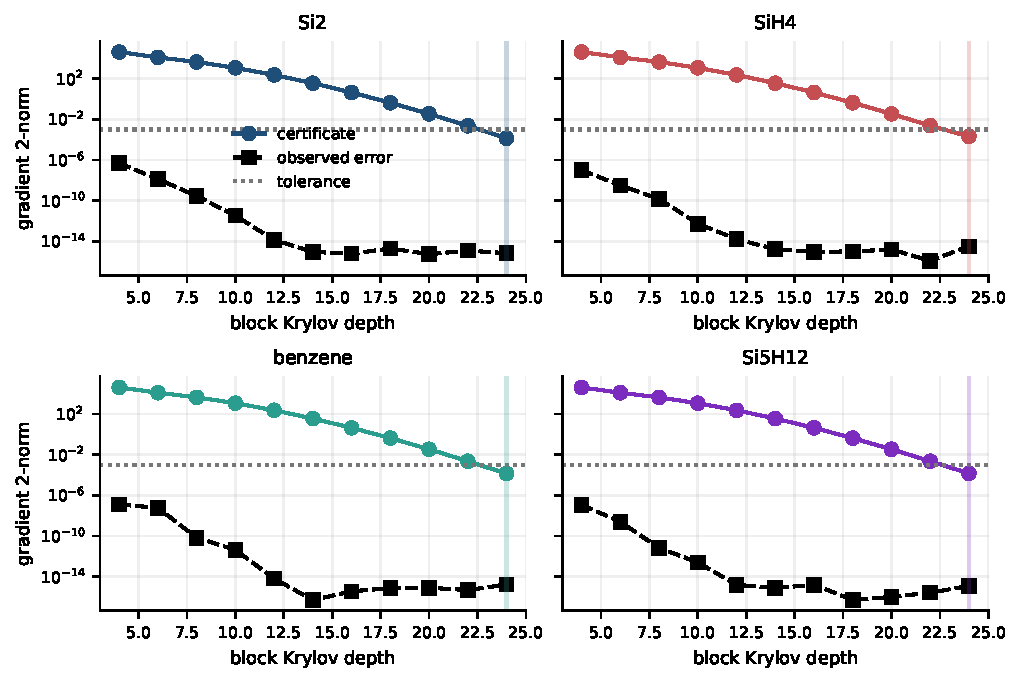
\includegraphics[width=.92\linewidth]{code/results/figures/certificate_frontier.pdf}
\caption{Joint-plan rank held fixed while depth varies. Preflight bounds and
independent-reference discrepancies are shown separately. The dotted line is
the primary tolerance; the vertical line marks certified selection.}
\label{fig:certificate}
\end{figure}
\begin{table}[htbp]
\centering\small
\caption{Matched observed and certified accuracy at $10^{-3}$. The observed
full-block choice is a post hoc minimum-work oracle on the tested grid.
Time ratio compares joint certification to that oracle; values above one
mean certification takes longer.}
\begin{tabular}{lrrrrr}\toprule matrix & $\norm g_2$ & joint work & certified full work & oracle work & time ratio\\\midrule
\MatchedRows\bottomrule\end{tabular}
\label{tab:matched}
\end{table}
\MatchedSummary{}
\begin{table}[htbp]
\centering\small
\caption{Rank-first budgets with the refined bounds. Entries are rank/depth/work;
the budget fraction assigns that fraction of $\varepsilon$ to compression.}
\begin{tabular}{lrrr}\toprule matrix & $0.05$ & $0.2$ & $0.5$\\\midrule
\PolicyRows\bottomrule\end{tabular}
\end{table}
\begin{table}[htbp]
\centering\small
\caption{Executable incremental full-rank adjoint baseline. The stopping rule
uses gradient agreement, while error is evaluated independently afterward.
The last column is the post hoc full-adjoint oracle's work, excluding its search
and reference cost. Runtime includes every checkpoint calculation.}
\label{tab:online}
\begin{tabular}{lrrrrrr}\toprule matrix & tolerance & depth & work & error & time (s) & oracle work\\\midrule
\OnlineRows\bottomrule\end{tabular}
\end{table}
\OnlineSummary{}
Absolute, relative, and normalized gradient-direction errors for each frontier
point are retained in the result record. The full gradient norms in
Table~\ref{tab:matched} make the absolute tolerance interpretable.

\begin{figure}[htbp]
\centering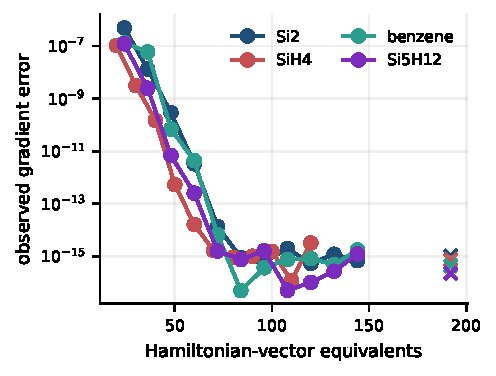
\includegraphics[width=.94\linewidth]{code/results/figures/work_accuracy.pdf}
\caption{Runtime versus discrepancy from the independent gradient. Curves show
selected-rank blocks, full blocks, a full-block projected adjoint, and scalar polarization at explicitly sampled
depths; stars show complete joint certification. Horizontal lines mark $10^{-3}$.
Points near the reference floor are numerical agreement, not proven absolute accuracy.}
\label{fig:frontiers}
\end{figure}
\begin{figure}[htbp]
\centering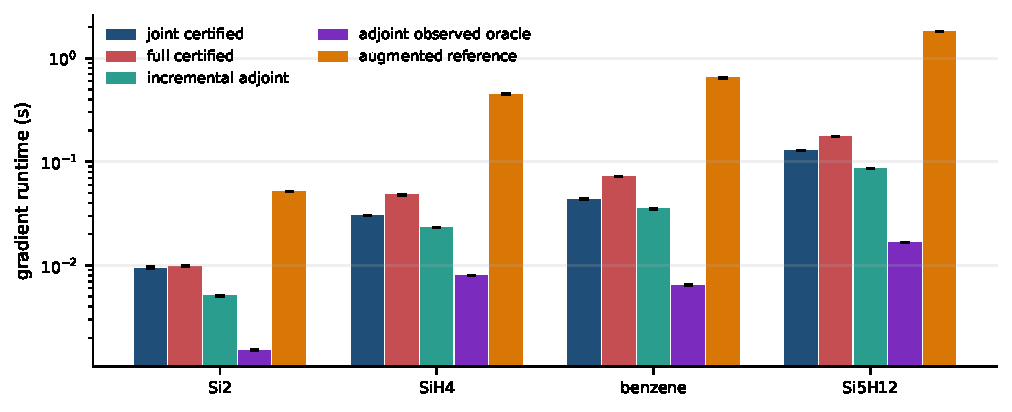
\includegraphics[width=.9\linewidth]{code/results/figures/runtime_scaling.pdf}
\caption{Per-matrix runtimes: joint certification, certified full rank,
incremental full adjoint, observed full-adjoint oracle at $10^{-3}$, and
independent augmented-exponential reference.
Bars show medians and whiskers the minimum--maximum repetition range.
The reference is an alternative numerical construction, not exact arithmetic.}
\label{fig:runtime}
\end{figure}

\subsection{Resource sensitivity and unfavorable probes}
\begin{figure}[htbp]
\centering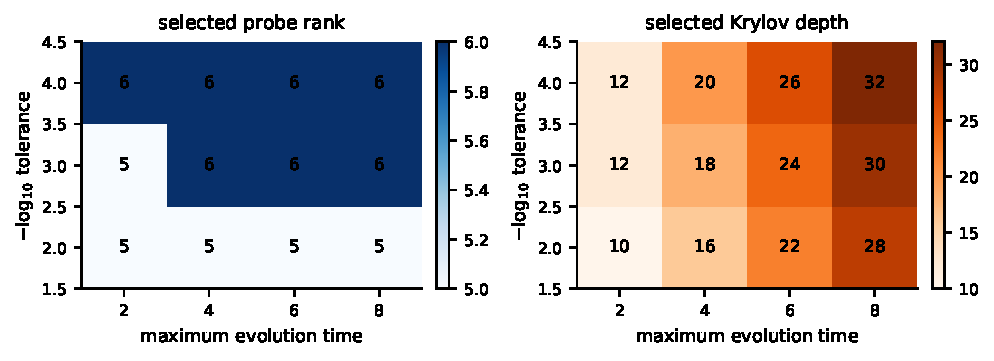
\includegraphics[width=.92\linewidth]{code/results/figures/rank_depth_map.pdf}
\caption{Joint rank--depth choices for the Si2 time--tolerance grid, using the
separate depth grid through 42. This is adaptation across inputs and tolerances,
not dependence on the current parameter at fixed inputs.}
\end{figure}
The 36 stress cases use symmetric tridiagonal matrices of order 80; block
widths $4,8,16$; one or six symmetric off-diagonal directions; horizons 2 or 8;
and probe singular values spanning 0, 1, or 3 decades. The tolerance is $10^{-5}$.
Independent augmented references are used in every case.
\StressSummary{}
These probes include orthogonal columns, so the study no longer tests only
strongly compressible input. Full-space reductions and numerical deflation are
counted by their actual applied widths. The result is a coverage and robustness
study, not evidence of large-scale performance for general sparse directions.

\subsection{Diagnostic recovery with the original certificate}
Consider a single particle on a 96-site open chain, with nearest-neighbor
adjacency $K$ and Hamiltonian
\begin{equation}
 A(\theta)=0.35I-0.22(1+0.3\theta_3)K
 +0.25\theta_1\operatorname{diag}(v_{30})
 +0.25\theta_2\operatorname{diag}(v_{60}),\quad
 (v_c)_i=e^{-(i-c)^2/(2\cdot7^2)}.
\end{equation}
Sites are indexed $0,\ldots,95$. Six normalized Gaussian wavepackets of width
6, centered at $24,26,28,56,58,60$, form the preparation block. Cosine block
entries are real transition amplitudes of $e^{-itA}$ for real preparations;
access requires coherent amplitude/interference measurements rather than only
transition probabilities. Here they are simulated without a device protocol.
The noise model adds symmetric Gaussian amplitude perturbations with scale
$10^{-4}$; it is not finite-shot or decoherence noise.

Two truths, $(0.22,-0.18,0.12)$ and $(-0.16,0.24,-0.14)$, are each fitted
from three starts: zero, $(-0.3,0.3,-0.25)$, and $(0.3,-0.25,0.3)$.
Training times are $(2,4,6)$ and held-out times are $(3,5,7)$.
Joint and full-rank certification use cached plans at successive tolerances
$10^{-3},10^{-5},10^{-7}$, with the original linear compression and Taylor
bounds retained for this control. Each stage runs L-BFGS-B on $[-0.5,0.5]^3$ with
at most 80 iterations; a depth-4 full-block baseline uses the same optimizer
schedule without certification. At a stage tolerance $\varepsilon$, its
projected-gradient threshold is $\varepsilon/10$, function tolerance is
$10^{-15}$, and at most 30 line-search trials are allowed. These settings
do not give an inexact-optimization convergence theorem. Optimizer status, every function-evaluation
trajectory, work, and elapsed time are stored. Each recovery is timed once;
variation across different starts is not a repeated-timing uncertainty estimate.
Final losses and held-out predictions are recomputed independently.

\begin{table}[htbp]
\centering\small
\caption{Simulated recovery: six runs per method and noise level (two truths,
three starts). Parameter error and held-out relative response error are maxima;
time is the median across those different runs. Recovery counts use parameter error below $10^{-3}$.}
\begin{tabular}{llrrrr}\toprule method & noise & recovered & max. param. error & held-out error & time (s)\\\midrule
\LearningRows\bottomrule\end{tabular}
\end{table}
\LearningSummary{}
\begin{table}[htbp]
\centering\small
\caption{Failed noiseless original-bound joint fits. The projected-gradient
residual is $\norm{\theta-\Pi_{[-.5,.5]^3}(\theta-g)}_2$ using an independent
gradient. The smallest Hessian eigenvalue is estimated by central differences
of independent gradients with step $10^{-5}$, only at interior fits.}
\begin{tabular}{lrrrr}\toprule estimate & param. error & loss & projected residual & min. eigenvalue\\\midrule
\FailureRows\bottomrule\end{tabular}
\end{table}
Small projected residuals at the incorrect boundary fits are compatible with
constrained stationarity. An incorrect interior fit with positive numerical
Hessian provides evidence of a nonglobal local minimum. Neither observation
proves the global structure of the inverse problem.
The observation Jacobian is formed independently at each truth. Its singular
values are retained, and \IdentifiabilitySummary{} This is local evidence only.
Cosine is even, so $A$ and $-A$ have identical responses whenever both are
admissible. The fixed positive diagonal and parameter box exclude that specific
sign reversal here; they do not prove global uniqueness. Successful runs also
do not establish global optimizer convergence.

\subsection{Larger learning problems with a feasible-direction test}
To exercise active compression, use open chains of $n=256$ and $1024$ sites,
with
\begin{equation}
 A(\theta)=0.7I-0.22(1+0.3\theta_3)K+
 0.18\theta_1\operatorname{diag}(w_{.25})+
 0.18\theta_2\operatorname{diag}(w_{.75}),\qquad
 (w_c)_i=e^{-(i/n-c)^2/(2\cdot.09^2)}.
\end{equation}
The parameter box remains $[-0.5,0.5]^3$. Twelve real preparations are the
normalized columns
\begin{equation}
 b_{c,k,a}(i)\ \propto\ e^{-\frac12((i-nc)/(.035n)-a)^2}\cos(ki),\qquad
 a\in\{-.12,-.04,.04,.12\}.
\end{equation}
The three center/carrier pairs are $(c,k)=(.25,0)$, $(.5,\pi/3)$, and
$(.75,\pi/2)$. Carrier wave numbers help separate sensitivity to
hopping and potential amplitudes. Lattice spacing, hopping, and time units
stay fixed while envelope widths grow with the chain; this is not a continuum
mesh-refinement experiment. The changed preparations, shorter times, and
larger positive diagonal define a separate, pilot-informed measurement design.
They are not an isolated ablation proving which change resolves the earlier
recovery failures.

Training times are $(1,2,3)$ and held-out times $(1.5,2.5,4)$. Three truths,
$(.22,-.18,.12)$, $(-.16,.24,-.14)$, and $(.08,.13,.23)$, use starts
$(0,0,0)$ and $(-.3,.3,-.25)$. Each has a noiseless data set and two
independent symmetric Gaussian amplitude-noise realizations of scale $10^{-4}$.
The complete factorial design crosses these settings with both sizes, four
methods, and stationarity targets $10^{-5}$ and $10^{-7}$. These remain
simulated coherent-amplitude observations, not finite-shot measurements.

All four methods use projected damped Gauss--Newton steps from the available
response derivatives, with a projected-gradient fallback. Joint and full
certification use the refined bounds, tightening tolerance until
Eq.~\eqref{eq:direction} is negative and the evaluated gradient-error bound
is at most one fifth of the projected-gradient norm. The stopping test adds
that bound to the projected-gradient norm and compares the sum to the
stationarity target. A full-rank depth-4 control and an independent
augmented-reference-gradient control use the same step and line-search
procedure without a gradient certificate. At most 35 accepted iterations and
20 backtracking trials per iteration are allowed.

Armijo acceptance uses independently computed sparse exponential actions of
the original loss for every method. These are floating-point evaluations;
we certify the feasible direction in exact arithmetic, not the complete
line search. All acceptance costs, norm-estimation and transpose actions are
counted. Final validation and a post hoc independent check of every computed
gradient are timed and counted separately from optimization. Reference
gradients do not influence the joint, full, or depth-4 directions. Stored
trajectories distinguish evaluation points from accepted iterates.

\begin{table}[htbp]
\centering\scriptsize
\caption{Larger learning study, with 18 runs per size, stationarity target,
and method. Recovery uses parameter error below $10^{-3}$. Rank and basis
dimension are ranges across all gradient evaluations, including tolerance
refinement; held-out error is the maximum. Time is the median full optimization
time including independent loss acceptance, excluding post hoc audits.}
\label{tab:scalable}
\begin{tabular}{rrlrrrrr}\toprule
$n$ & stopping target & method & recovered & rank & basis dim. & held-out error & time (s)\\\midrule
\ScalableRows\bottomrule\end{tabular}
\end{table}
\ScalableSummary{}
\begin{table}[htbp]
\centering\small
\caption{Joint/full learning cost at each size and stopping target. Work
entries are medians across the same 18 cases, in joint/full order. Total
Hamiltonian work includes independent loss acceptance during optimization;
post hoc audit work is excluded. The last column is joint/full median runtime.}
\label{tab:learning-cost}
\begin{tabular}{rrrrr}\toprule
$n$ & stopping target & Krylov work & total Hamiltonian work & time ratio\\\midrule
\ScalableCostRows\bottomrule\end{tabular}
\end{table}
At the looser stopping target, joint selection lowers the median Krylov work
from 504 to 396, but the independent acceptance actions reduce the saving in
total Hamiltonian work. At the stricter target, repeated refinement raises
joint Krylov work to 792 versus 672 for full certification. Joint selection
is slower than full certification in all four size/tolerance groups, and the
depth-4 control remains faster. Active compression and successful recovery
therefore establish feasibility, not a net speed advantage. All methods
reach the requested independent projected-stationarity threshold. The reduced
matrices occupy fewer than $n$ columns throughout; basis storage is recorded,
but peak process memory is not measured.
\begin{figure}[htbp]
\centering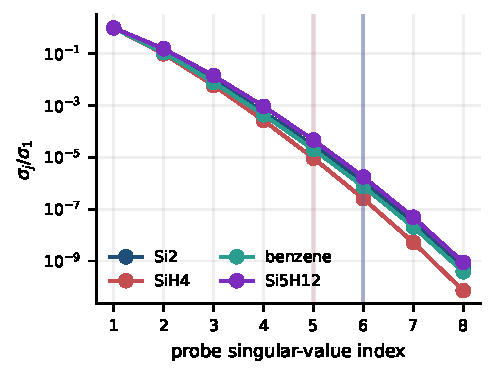
\includegraphics[width=.95\linewidth]{code/results/figures/probe_spectrum.pdf}
\caption{Larger learning at stationarity target $10^{-7}$. Left: accepted
iterates for the first noiseless truth and zero start at each size. Right:
all 18 final results per method, including both noise realizations and both
starts. Optimization times include independent loss acceptance; audit time
is excluded. Parameter error is evaluated against the generating truth.}
\label{fig:learning}
\end{figure}

\section{Limitations and conclusion}
The method provides an exact-arithmetic gradient bound and a finite-grid work
optimum. Upward rounding of the tail evaluation does not certify row sums,
SVD truncation, the computed basis, reduced eigensystems, or gradient assembly.
The reported errors are discrepancies from an independently implemented
floating-point reference. High-precision or interval end-to-end certification
remains outside the present implementation.

The comparisons expose the main practical limitation: even the refined
certificate can require substantially more depth than observed accuracy needs.
A compressed certified computation must therefore be judged against certified
and uncertified alternatives separately. Spectrum-adapted bounds
\cite{xu2022,chen2022,simunec2023} and a cost model incorporating orthogonalization
may further improve selection. The incremental and projected-adjoint controls
strengthen the executable comparisons, but they are not an exhaustive
state-of-the-art study. The tight-binding studies are simulated; their success
or failure cannot be extrapolated to device
Hamiltonian identification \cite{shabani2011,wiebe2014,bairey2019}.

The resulting contribution is a reproducible study of the benefits and costs of
certifying block matrix-function gradients. It supplies actual parameter
recovery and independent references while preserving unfavorable cases.
Practical usefulness depends on probe correlation, required accuracy, and
whether a deterministic bound is itself an application requirement.

\section{Data and code availability}
Source, tests, pinned matrix checksums, complete numerical records, and figure
scripts are in the accompanying repository at
\url{https://github.com/thmolena/Block-Matrix-Products-for-Quantum-Operator-Learning}.
Reproduction and validation commands are given in the repository README. The
implementation SHA-256 digest begins \ImplementationDigest{} and identifies
the executable source and dependency specification; its full value is stored
with the results. The timing-independent numerical digest begins
\SemanticDigest{}. It detects changes in rounded numerical content, not
scientific validity. External archives are downloaded, not redistributed.
No archival DOI is claimed for this revision.

\FloatBarrier
\appendix
\section{Positive tail evaluation}
Let $q$ be the first even integer greater than $d$, and $z=|t|\rho$.
Successive even response terms have ratio at most
$\zeta_0=z^2/((q+1)(q+2))$; derivative terms have ratio at most
$\zeta_1=z^2/(q(q+1))$. If the relevant ratio is below one,
\begin{equation}
 R_d^{(0)}\le\frac{z^q}{q!(1-\zeta_0)},\qquad
 R_d^{(1)}\le\frac{q|t|^q\rho^{q-1}}{q!(1-\zeta_1)}.
\end{equation}
Otherwise the implementation marks that tail infeasible and advances the depth.
The formulas use 80-digit decimal arithmetic followed by an upward binary64
conversion. Response and derivative tails use their own degrees. The numerical
implementation is not a full interval-arithmetic evaluation of the theorem.
For the Chebyshev tails let $a=z/2$ and $b_q=2a^q/q!$. Their successive-term
ratios are bounded by
$\xi_0=a^2/((q+1)(q+2))$ and
$\xi_1=a^2(q+2)/(q^2(q+1))$, giving
\begin{equation}
 E_d^{(0)}\le\frac{b_q}{1-\xi_0},\qquad
 E_d^{(1)}\le\frac{q^2b_q}{\rho(1-\xi_1)}.
\end{equation}
An invalid denominator marks only that tail infeasible. Compared with the
Taylor majorants, the first omitted response term shrinks by $2/2^q$, the
derivative term by $2q/2^q\le1$, and both ratios decrease. Thus this tail
refinement is never worse under the same enclosure and polynomial degree.

\section{Independent references and checks}\label{sec:reference}
For $p$ directions, assemble a sparse block lower-triangular matrix $\mathcal A$
with $A$ on each of its $p+1$ diagonal blocks and $D_j$ in block $(j+1,1)$.
Applying $e^{-it\mathcal A}$ to $(B,0,\ldots,0)^{\mathsf T}$ produces
$e^{-itA}B$ in its first block and the exponential Fr\'echet actions in the
remaining blocks \cite{vanloan1978,al-mohy2009}. Their real parts give cosine
responses and derivatives. SciPy's exponential-action algorithm operates on
this sparse augmented matrix; it does not use the projected cosine routine.
The augmented problem has dimension $(p+1)n$ and is timed separately.

Tests compare clustered-eigenvalue divided differences and off-diagonal
projected gradients with an independent dense exponential Fr\'echet routine.
Explicit monomial sums check both exactness degrees and exhibit failure beyond
the derivative degree. An exhaustive enumeration checks the discrete joint
work minimum. The Si2--Si5H12 depth-28 reference discrepancies are additionally
recorded against the augmented construction; depth agreement alone is not
used as an independent validation argument.
\FloatBarrier

\begin{thebibliography}{99}

\bibitem{dlmf}
NIST Digital Library of Mathematical Functions, Sections 10.12 and 10.14,
Eqs.~10.12.3 and 10.14.4, \url{https://dlmf.nist.gov/10.14.E4}
(accessed September 15, 2026).

\bibitem{higham2008}
N. J. Higham, \textit{Functions of Matrices: Theory and Computation}
(SIAM, Philadelphia, 2008), doi:10.1137/1.9780898717778.

\bibitem{saad1992}
Y. Saad, Analysis of some Krylov subspace approximations to the matrix
exponential operator, SIAM J. Numer. Anal. \textbf{29}, pp.~209--228 (1992),
doi:10.1137/0729014.

\bibitem{hochbruck1997}
M. Hochbruck and C. Lubich, On Krylov subspace approximations to the matrix
exponential operator, SIAM J. Numer. Anal. \textbf{34}, pp.~1911--1925 (1997),
doi:10.1137/S0036142995280572.

\bibitem{lanczos1950}
C. Lanczos, An iteration method for the solution of the eigenvalue problem of
linear differential and integral operators, J. Res. Natl. Bur. Stand.
\textbf{45}, 255 (1950).

\bibitem{golub2010}
G. H. Golub and G. Meurant, \textit{Matrices, Moments and Quadrature with
Applications} (Princeton University Press, Princeton, 2010).

\bibitem{gutknecht2007}
M. H. Gutknecht, Block Krylov space methods for linear systems with multiple
right-hand sides: an introduction, in \textit{Modern Mathematical Models,
Methods and Algorithms for Real World Systems}, edited by A. H. Siddiqi,
I. S. Duff, and O. Christensen (Anamaya, New Delhi, 2007), pp. 420--447.

\bibitem{xu2022}
Q. Xu and T. Chen, A posteriori error bounds for the block-Lanczos method for
matrix function approximation, Numer. Algorithms \textbf{98}, pp.~903--927
(2025), doi:10.1007/s11075-024-01819-7.

\bibitem{kandolf2017}
P. Kandolf and S. D. Relton, A block Krylov method to compute the action of the
Fr\'echet derivative of a matrix function on a vector with applications to
condition number estimation, SIAM J. Sci. Comput. \textbf{39}, pp.~A1416--A1434 (2017),
doi:10.1137/16M1077969.

\bibitem{kandolf2021}
P. Kandolf, A. Koskela, S. D. Relton, and M. Schweitzer, Computing low-rank
approximations of the Fr\'echet derivative of a matrix function using Krylov
subspace methods, Numer. Linear Algebra Appl. \textbf{28}, e2401 (2021).

\bibitem{kressner2019}
D. Kressner, A Krylov subspace method for the approximation of bivariate matrix
functions, in \textit{Structured Matrices in Numerical Linear Algebra}
(Springer, Cham, 2019), pp. 197--214.

\bibitem{singh2026}
N. Singh, K. Barros, and X. S. Li, Fast and stable gradient approximation for
bilinear forms of Hermitian matrix functions, arXiv:2605.12801 (2026).

\bibitem{al-mohy2009}
A. H. Al-Mohy and N. J. Higham, Computing the Fr\'echet derivative of the matrix
exponential, with an application to condition number estimation,
SIAM J. Matrix Anal. Appl. \textbf{30}, pp.~1639--1657 (2009), doi:10.1137/080716426.

\bibitem{davis2011}
T. A. Davis and Y. Hu, The University of Florida Sparse Matrix Collection,
ACM Trans. Math. Softw. \textbf{38}, 1 (2011).

\bibitem{chel1994}
J. R. Chelikowsky, N. Troullier, and Y. Saad, Finite-difference-pseudopotential
method: Electronic structure calculations without a basis, Phys. Rev. Lett.
\textbf{72}, 1240 (1994).

\bibitem{chen2022}
T. Chen, A. Greenbaum, C. Musco, and C. Musco, Error bounds for Lanczos-based
matrix function approximation, SIAM J. Matrix Anal. Appl. \textbf{43}, pp.~787--811 (2022),
doi:10.1137/21M1427784.

\bibitem{simunec2023}
I. Simunec, Error bounds for the approximation of matrix functions with rational
Krylov methods, arXiv:2311.02701 (2023).

\bibitem{beckermann2018}
B. Beckermann, D. Kressner, and M. Schweitzer, Low-rank updates of matrix
functions, SIAM J. Matrix Anal. Appl. \textbf{39}, pp.~539--565 (2018), doi:10.1137/17M1140108.

\bibitem{higham2014}
N. J. Higham and S. D. Relton, Higher order Fr\'echet derivatives of matrix
functions and the level-2 condition number, SIAM J. Matrix Anal. Appl. \textbf{35}, pp.~1019--1037
(2014), doi:10.1137/130945259.

\bibitem{rubensson2024}
E. H. Rubensson, A unifying framework for higher order derivatives of matrix
functions, SIAM J. Matrix Anal. Appl. \textbf{45}, pp.~504--528 (2024),
doi:10.1137/23M1580589.

\bibitem{vanloan1978}
C. F. Van Loan, Computing integrals involving the matrix exponential, IEEE
Trans. Autom. Control \textbf{23}, 395 (1978).

\bibitem{shabani2011}
A. Shabani, R. L. Kosut, M. Mohseni, H. Rabitz, M. A. Broome,
M. P. Almeida, A. Fedrizzi, and A. G. White, Efficient measurement of quantum
dynamics via compressive sensing, Phys. Rev. Lett. \textbf{106}, 100401 (2011).

\bibitem{wiebe2014}
N. Wiebe, C. Granade, C. Ferrie, and D. G. Cory, Hamiltonian learning and
certification using quantum resources, Phys. Rev. Lett. \textbf{112}, 190501
(2014).

\bibitem{bairey2019}
E. Bairey, I. Arad, and N. H. Lindner, Learning a local Hamiltonian from local
measurements, Phys. Rev. Lett. \textbf{122}, 020504 (2019).

\bibitem{cramer2010}
M. Cramer, M. B. Plenio, S. T. Flammia, R. Somma, D. Gross,
S. D. Bartlett, O. Landon-Cardinal, D. Poulin, and Y.-K. Liu,
Efficient quantum state tomography, Nat. Commun. \textbf{1}, 149 (2010).

\bibitem{childs2017}
A. M. Childs, D. Maslov, Y. Nam, N. J. Ross, and Y. Su,
Toward the first quantum simulation with quantum speedup,
Proc. Natl. Acad. Sci. USA \textbf{115}, 9456 (2018).

\end{thebibliography}
\end{document}
